\subsection{Анализ формата входных данных}

С заданной периодичностью, циклически маячок выдает один и тот же набор данных \cite{web:HabrBig, web:HabrIOS7}:

\begin{figure}[h!]
    \centering
    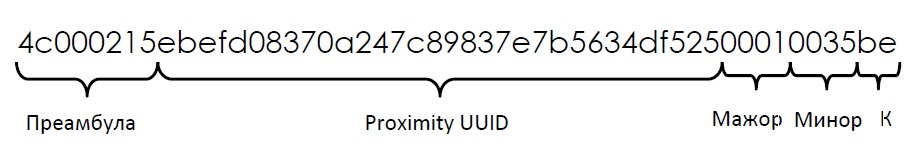
\includegraphics[width=\textwidth]{img/packageData2}
    \caption{Пример пакета, передаваемого маячком}
    \label{params}
\end{figure}

\begin{figure}[h!]
    \centering
    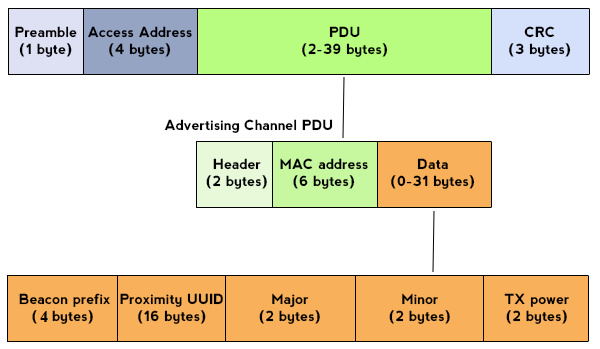
\includegraphics[width=\textwidth]{img/packageStructure}
    \caption{Общая структура Bluetooth-пакета}
\end{figure}

\textbf{Преамбула (4 байта)} - префикс пакета, позволяющий установить, что мы имеем дело именно с Beacon-маячком. Всегда равен \texttt{4c000215}. Преамбула состоит из 4-х полей: идентификатор компании (2 байта, в данном примере - \texttt{4c00}), тип (1 байт, в примере - \texttt{0x02}) и длина данных (1 байт, значение - \texttt{0x15}).

\textbf{Proximity UUID (16 байт)} – Идентификатор группы маяков. Например, если существуют несколько торговых залов, в которых требуется разместить маяки, то во всех этих залах они будут иметь один и тот же UUID, указанный при конфигурации, и это позволит отличать маяки от других, посторонних.

\textbf{Мажор (2 байта)} – позволяет различать небольшой набор маяков внутри одной группы. То есть внутри одной большой группы маяков, идентифицируемой UUID, может быть несколько подгрупп, каждая из которых идентифицируется по номеру мажора. Например, согласно приведенному выше примеру, каждому залу можно присвоить свой номер мажора. Если маяками требуется охватить несколько этажей здания - обычно с каждым этажом ассоциируют свой номер мажора.

\textbf{Минор (2 байта)} – номер, идентифицирующий сам маяк внутри мажора. Связка uuid+мажор+минор позволяет нам однозначно идентифицировать маяк и по этим данным определить координату самого маячка (обычно используется таблица соответствия маячка и его координат).

\textbf{TX Power (параметр K на рисунке выше, 2 байта)} – эталонное значение мощности маячка, представляющее собой силу сигнала на расстоянии в 1 метр от маячка и измеряется в децибелах. Измеряется это единственный раз при изготовлении маячка и вшивается в него изначально. Сравнивая эталонное значение мощности и текущее, получаемое в процессе работы, возможно вычислить расстояние до источника сигнала. Первый бит является знаковым (1 - <<$-$>>, 0 - <<$+$>>). Например, TX Power в нашем примере (см. рисунок \ref{params}, параметр <<К>>) – \texttt{0xBE}, то есть 190 в десятичной системе счисления. Тогда эталонная сила сигнала на расстоянии 1м от маячка составляет $256-190=-66$ dBm.